\documentclass[11pt]{article}

\usepackage[margin=1.15in]{geometry}
\usepackage{amsmath,amssymb,amsthm,mathtools}
\usepackage{booktabs,array,tabularx,longtable}
\usepackage{graphicx}
\usepackage{xcolor}
\usepackage{enumitem}
\usepackage{microtype}
\usepackage[hidelinks]{hyperref}
\usepackage{caption}
\captionsetup{font=small,labelfont=bf}
\setlength{\parskip}{0.55em}
\setlength{\parindent}{0pt}
\renewcommand{\arraystretch}{1.18}

% status tags
\newcommand{\stR}{\textbf{\textcolor{blue!55!black}{[R]}}}
\newcommand{\stA}{\textbf{\textcolor{orange!70!black}{[A]}}}
\newcommand{\stD}{\textbf{\textcolor{green!40!black}{[D]}}}
\newcommand{\stP}{\textbf{\textcolor{violet!80!black}{[P]}}}

\newcommand{\thz}{\,\mathrm{THz}}
\newcommand{\kjm}{\,\mathrm{kJ\,mol^{-1}}}
\newcommand{\cmi}{\,\mathrm{cm^{-1}}}

\theoremstyle{plain}
\newtheorem{proposition}{Proposition}
\newtheorem{criterion}{Criterion}
\theoremstyle{definition}
\newtheorem{definition}{Definition}
\theoremstyle{remark}
\newtheorem{remark}{Remark}

\title{Resonance Without Regulation:\\[0.3em]
Quantum Interpretation and Functional Inference\\[0.2em]
in Mitochondrial Biology}
\author{Flyxion\\ \small Independent Researcher}
\date{October 2026}

\begin{document}
\maketitle

\begin{abstract}
\noindent A recent preprint reports an infrared spectral shoulder near 71.0\,THz in living cells and tissues, proposes that it is the lower branch of a light--matter hybrid excitation of lipid CH$_2$ vibrations in mitochondrial cristae, and reports an increase of about ten percent in measured ATP after ten minutes of low-power illumination at 71 and 87\,THz. This essay uses the preprint as a concrete case for a general question: what does a demonstrated response to an intervention license one to conclude about mechanism, function, and control? The analysis separates four levels of claim (spectral observation, physical mechanism, biological function, and selective control) and labels every statement as reported, assumed, deduced, or proposed. Four results are developed. First, an audit of the coupled-mode model shows that the stated coupling strength of $6.4\kjm$ is not fixed by the inputs the preprint reports: the stated CH$_2$ density is inconsistent with the stated bond spacing by almost four orders of magnitude, an oscillator-strength consistency constraint, evaluated with order-of-magnitude hydrocarbon absorption values that are flagged as unsourced, implies a collective coupling of order one terahertz rather than sixteen, and the model evaluated at its own stated geometry predicts tissue-dependent branch positions that differ from the single reported value. Second, a formal treatment shows that one response of one measured variable to one stimulus establishes neither selectivity, independent controllability, nor endogenous utilization. Third, a comparison with quantum-like two-state models of bistable perception shows that formal equivalence of two-state Hamiltonians does not imply mechanistic equivalence, and that even a verified avoided crossing would establish a hybrid normal mode that linear response also describes classically. Fourth, counterfactual experiments are developed, centred on a structurally induced shift of the resonance and on isotopic substitution of the acyl chains, that separate a mechanism that predicts new observations from one that accommodates existing ones. The analysis is not a rejection of quantum biology, and both the spectral measurements and the illumination result merit replication.
\end{abstract}

\section{Scope, Sources, and Conventions}

The subject is the preprint by Yang, Gu, and Song, \emph{A quantum state of mitochondria in the living cell}, posted to bioRxiv on 15 September 2026 (doi:10.64898/2026.09.10.750628) and not peer reviewed at the time of writing. The 33-page PDF, including Supplementary Figures 1 to 11, was read in full, and page numbers below refer to that file. The main text refers to further detail in a Supplementary Information section, but the file contains only the supplementary figures. Items such as spectral resolution, scan count, and the line-shape model used in the multipeak fits are therefore described here as not stated in the material examined, which is a statement about the file and not about the underlying laboratory records.

The purpose of the essay is methodological. The preprint is a useful case because it contains, within a few pages, a measurement, a model, a perturbation experiment, and a verbal escalation from each to the next. It is also a case in which most of the individual components are physically reasonable. Polariton physics is a legitimate framework for collective molecular excitations, infrared spectroscopy of living material is difficult and worth doing, and low-power mid-infrared illumination of cells is an active research topic. The question is what each piece of evidence supports, and the aim is to state that precisely enough that a replication or a refutation would be recognizable as such. Nothing here is a categorical rejection of quantum effects in biology; the conclusion is that this particular chain of inference is underdetermined at several links, and that the most informative next experiments are ones the proposed mechanism itself implies.

Because the argument depends on keeping the provenance of statements visible, every empirical, quantitative, or inferential claim about the preprint or its model carries one of four tags, used consistently and collected in the ledger of Section~\ref{sec:ledger}. Framing, definitional, and purely mathematical statements (the propositions and their proofs, which depend only on their stated hypotheses) are left untagged, and untagged expository text makes no independent claim about the preprint.

\begin{itemize}[leftmargin=2.2em,itemsep=0.2em]
\item[\stR] \emph{Reported}: a measurement or statement that appears in the preprint, with its location.
\item[\stA] \emph{Assumed}: a modelling choice or interpretive premise adopted by the authors without independent demonstration in the preprint.
\item[\stD] \emph{Deduced}: a conclusion derived here from \stR{} and \stA{} items together with standard physics, with the inputs listed. Deductions are audits under stated inputs, and where an input is not reported in the preprint a range is used and said to be a range.
\item[\stP] \emph{Proposed}: an experiment or criterion suggested here, not performed by anyone.
\end{itemize}

\section{Four Levels of Claim}
\label{sec:levels}

The preprint moves between statements of different logical strength, and it helps to name them. Four levels are distinguished. The first is a \emph{spectral observation}: an absorption feature at about $71.0\thz$ is present in attenuated-total-reflectance spectra of living preparations. The second is a \emph{physical mechanism}: the feature is the lower branch of a hybrid excitation formed by collective coupling between lipid CH$_2$ stretching vibrations and a confined infrared photon mode in mitochondrial cristae. The third is a \emph{biological function}, which itself divides into two claims that are often run together. The first of these, \emph{exogenous response}, is that ATP abundance changes when cells are illuminated at the relevant frequencies. The second, \emph{endogenous utilization}, is that cells ordinarily use the proposed mode in regulating energy metabolism. The fourth level is \emph{selective control}: stimulation at the mode frequency is a channel through which ATP can be regulated specifically, within stated operating limits and independent of the initial physiological state.

Table~\ref{tab:levels} places the preprint's claims against these levels. The point of the table is not that the lower levels are weak. The first is a reported measurement that can be checked by others. The point is that evidence for one level does not transfer upward automatically. Failure at a lower level defeats the claims above it, but success at a lower level only makes the higher claim possible. This asymmetry is the same one examined in a companion essay on enabling conditions and demonstrated function, where a physically permitted arrangement is distinguished from a function that has been shown to occur. The preprint is a clean instance because the mechanism is introduced precisely as an enabling condition (a geometry that would permit coupling) and then read as a realized function.

\begin{table}[ht]
\centering
\small
\begin{tabularx}{\textwidth}{@{}p{2.5cm}XX@{}}
\toprule
Level & What the preprint offers & Evidential status \\
\midrule
1. Spectral observation & Shoulder at 71.0\,THz in ATR spectra of HEK-293T cells and four mouse tissues, and in isolated mitochondria; absent in dried, KBr-pellet transmission spectra (pp.~4--6, Figs.~1--2) & Measured. Decomposition from a nearby gas-phase CO$_2$ band rests on multipeak fitting; preparations differ in several variables at once (Section~\ref{sec:obs}). \\
2. Physical mechanism & Coupled-mode Hamiltonian, Eqs.~1--6 (pp.~9--10); cavity argument $L=m\lambda_m/2$ (pp.~8, 10--11, Fig.~4) & Proposed model. Parameters not independently measured; several internal inconsistencies (Section~\ref{sec:model}). \\
3a. Exogenous response & ATP per cell $+10.3\%$ at 71\,THz, $+10.1\%$ at 87\,THz, no significant change at 53.7\,THz; $n=8$ paired wells (pp.~11--12, Fig.~5) & Measured as endpoint abundance after lysis. Production is not separated from consumption (Section~\ref{sec:atp}). \\
3b. Endogenous utilization & Posed as an open question about energy metabolism and ``information transmission'' (abstract, p.~12) & No data. \\
4. Selective control & Language of an ``efficient channel'' to modulate ATP (pp.~1, 12) & Not tested: no response function, off-target coordinates, or state dependence (Section~\ref{sec:control}). \\
\bottomrule
\end{tabularx}
\caption{Claims in the preprint arranged by level, with the evidence offered at each.}
\label{tab:levels}
\end{table}

\section{The Record: What Is Reported and What Is Assumed}
\label{sec:record}

A compact record of what the preprint states prevents later sections from drifting into a different paper than the one under examination. The measured items are as follows. \stR{} Living HEK-293T cell pellets, mouse kidney, liver, heart and skeletal muscle, and mitochondria isolated from these were measured by FTIR in ATR mode with a BaF$_2$ powder suspension in water as background; dried samples (65\,$^\circ$C oven, ground with KBr at 1:200, pressed) were measured in transmission mode under nitrogen purge (Methods, p.~13; Supplementary Figs.~8--9). \stR{} A group of peaks between 68.5 and 70.4\,THz is assigned to dissolved CO$_2$, the main peak at 70.8\,THz to gaseous CO$_2$, and a shoulder at 71.0\,THz is left unassigned, with multipeak fits reported at $R^2>0.995$ (p.~5, Figs.~1--2). \stR{} Mitochondrial length from JC-1 confocal imaging is $2.2\pm0.4\,\mu\mathrm{m}$ ($n=100$) for HEK-293T cells, kidney, and liver, and $1.2\pm0.2\,\mu\mathrm{m}$ for heart and skeletal muscle (pp.~7, 10--11, Fig.~4a). \stR{} ATP was measured by luciferase assay on lysates of Matrigel cell clusters of about 1\,mm, after 10 minutes of illumination at a stated 10\,$\mu$W per mm$^2$ with 10\,$\mu$W at the fibre tip, in an incubator at 37\,$^\circ$C and 5\% CO$_2$, using paired untreated wells and a paired $t$-test (pp.~11--14, Fig.~5, Supplementary Figs.~10--11).

The assumptions on which the interpretation rests are the following. \stA{} The lipid CH$_2$ stretching mode at 87\,THz and a standing-wave photon mode at the same frequency are in exact resonance, supported by the observation that $L_m\approx\lambda_m$ or $\lambda_m/2$ with $\lambda_m=\lambda_0/n$ and $n\approx1.5$ (pp.~8, 10). \stA{} The mitochondrion can be treated as a one-dimensional cavity along its axis, with emitted photons propagating along the axis (pp.~8--9). \stA{} The direction-matching factor $\eta_k\to1$ for energy-active mitochondria (p.~10). \stA{} The coupling strength is obtained from the collective expression of Eq.~4, with the CH$_2$ density quoted on p.~8; no value of the transition dipole is reported in the main text. \stA{} The upper branch at 103\,THz is not resolvable because it falls within the 90--110\,THz range of amide A and water absorption (p.~10). \stA{} No molecular vibration contributes in the 60--80\,THz range, based on spectra reproduced from earlier literature (Supplementary Fig.~1, p.~23). \stA{} The disappearance of the feature in dried, ground samples reflects collapse of cristae structure, $t_k\to0$ (p.~10).

Two features of the preprint's own wording deserve fairness. The abstract and conclusion state that the authors ``demonstrate'' a quantum state, but the same conclusion describes the calculations as having ``suggested'' it, and the question of whether the state could act as a channel for energy metabolism and information transmission is presented as a direction for further exploration (p.~12). The analysis below therefore treats the headline wording as stronger than the body in places, and does not attribute to the authors claims they framed as open.

\section{The Spectral Observation}
\label{sec:obs}

\subsection{Separation from a neighbouring gas-phase band}

\stR{} The unassigned shoulder at 71.0\,THz sits $0.2\thz$ above the 70.8\,THz peak that the authors assign to gaseous CO$_2$ (p.~5). \stD{} In spectroscopic units this is $0.2\thz = 6.7\cmi$, since $1\thz = 33.36\cmi$. \stR{} The spectral resolution, scan number, apodization, and the line-shape and baseline model of the multipeak analysis are not stated in the main text or the supplementary figures supplied. \stD{} A separation of $6.7\cmi$ is of the same order as resolutions commonly used in biological FTIR work, a few wavenumbers, so the shoulder lies near the limit of what the sampling can separate, although the actual setting is unreported.

A coefficient of determination above 0.995 measures how well a sum of fitted components reproduces the measured curve. It does not measure whether the decomposition is unique. For a model $S(\nu)=\sum_j a_j\,\varphi(\nu;\nu_j,\Gamma_j)+b(\nu)$ with line shapes $\varphi$ and a baseline $b$, the information that the data carry about a weak component close to a stronger one degrades as the separation falls below the linewidth, because the columns of the Jacobian with respect to the two amplitudes become nearly collinear. In that regime different line-shape choices, baseline polynomials, and numbers of components achieve essentially identical $R^2$ while assigning different weights to the shoulder. \stP{} The stability of the 71.0\,THz component should therefore be reported under alternative line shapes (Gaussian, Lorentzian, Voigt), alternative baselines, and varying numbers of CO$_2$(aq) components, together with parameter uncertainties and a blinded decomposition.

\subsection{A contrast between preparations is not a contrast in one variable}

\stR{} The comparison that carries the claim that the feature requires intact structure is between living material in ATR mode and dried, ground material in KBr transmission under nitrogen purge. \stD{} Treat this as an intervention on a bundle of factors $Z$ (viability, hydration, tissue organization, chemical environment, optical geometry, and atmosphere), all of which differ between arms. The experiment then identifies the effect of the bundle. Attributing the effect to the single component ``mitochondrial structural integrity'' requires variation in that component with the rest of $Z$ held fixed.

\begin{proposition}[Contrast versus variable]
\label{prop:contrast}
Let $T\in\{0,1\}$ index two preparations that differ in a vector of factors $Z=(Z_1,\dots,Z_k)$, and let a feature $F$ be present for $T=1$ and absent for $T=0$. Then the data are consistent with the proposition that $F$ depends on $Z_i$ and not on $Z_j$ for any chosen pair $i\ne j$.
\end{proposition}

\begin{proof}
The observation fixes only the value of $F$ on two points of the factor space, $z_0$ and $z_1$, which differ in every coordinate. Define $F(z)=\mathbf 1[z_i=z_{1,i}]$. This agrees with the data and ignores every other coordinate. Exchanging $i$ for $j$ gives an equally consistent function.
\end{proof}

The proposition is elementary, but it identifies what additional design would be informative. \stD{} One difference that is not incidental is the atmosphere. The preprint states that the dried samples were measured under nitrogen purge, and it reports no purge for the ATR measurements of living material. \stR{} The authors themselves assign the main 70.8\,THz peak of the living spectra to gas-phase CO$_2$, and a CO$_2$ reference spectrum recorded by ATR shows the same peak (Supplementary Fig.~2), so the living spectra contain an ambient-air CO$_2$ contribution at the frequency of the new shoulder. \stD{} The asymmetric-stretch band of gas-phase CO$_2$ has its origin near $2349\cmi$ (about 70.4\,THz) with a rotational R branch at higher wavenumber, and $71.0\thz$ corresponds to $2368\cmi$. This is spectroscopic background knowledge and not a result of the preprint, and it should be checked against a gas-phase reference at matched resolution, but it indicates that the shoulder lies inside the spectral region occupied by the high-frequency side of that band. The purge differs between the arms, and a shoulder on the side of a band whose shape depends on resolution, path, and background subtraction is the kind of feature that a difference in atmosphere can create or remove.

\stP{} Three experiments would separate the candidate variables. First, measure living material by ATR under nitrogen purge, and measure disrupted material (graded sonication or detergent permeabilization) by ATR at fixed hydration in the same atmosphere, so that structural integrity varies while hydration, geometry, and atmosphere do not. Second, replace the CO$_2$ source by $^{13}$CO$_2$ and $^{13}$C-bicarbonate. The $^{13}$C asymmetric stretch lies about $66\cmi$ (roughly 2\,THz) lower, so a shoulder derived from any form of CO$_2$ should move with the label, while a shoulder derived from lipid CH$_2$ should not. Third, repeat the measurement of isolated mitochondria with osmotic or detergent disruption titrated against a functional readout, so that the feature can be followed as a function of a continuous structural variable and not a binary contrast.

\section{The Coupled-Mode Model}
\label{sec:model}

\subsection{Algebra of the two-mode Hamiltonian}

\stR{} The preprint writes the Hamiltonian as $H=\sum_k H_{0,k}+H_{\mathrm{int},k}$ with a cavity-photon mode of energy $h\nu_k$, a collective CH$_2$ vibron of energy $\hbar\omega_{\mathrm{vib}}$, and an interaction of the exchange form $t(B^\dagger b+b^\dagger B)$ (Eqs.~1--3, p.~9). In the single-photon, single-vibron sector this is the two-by-two matrix
\begin{equation}
H_k=\begin{pmatrix} h\nu_k & t_k\\ t_k & h\nu_{\mathrm{vib}}\end{pmatrix},
\end{equation}
with eigenvalues
\begin{equation}
E_k^{\pm}=\frac{h\nu_k+h\nu_{\mathrm{vib}}}{2}\pm\sqrt{\Bigl(\frac{h\nu_k-h\nu_{\mathrm{vib}}}{2}\Bigr)^{2}+t_k^{2}},
\label{eq:branches}
\end{equation}
which is the paper's Eq.~5, and at resonance $E^{\pm}=h\nu_{\mathrm{vib}}\pm t_k$ (Eq.~6). \stD{} The algebra is correct. \stR{} The authors take $\nu_{\mathrm{vib}}=87\thz$ and $t_k\approx6.4\kjm$ and obtain branches at 71 and 103\,THz (p.~10). \stD{} With $h=0.399\kjm\thz^{-1}$, a coupling of $6.4\kjm$ is $16.04\thz$, so the branches are $87\mp16.04\thz=70.96$ and $103.04\thz$, and the splitting is $2t=32\thz$. The consistency of the arithmetic is not in question. The question is whether the inputs are determined independently of the feature the model is meant to explain.

\stD{} One observation is relevant here. The quoted coupling $t\approx6.4\kjm$ equals, to the precision stated, exactly the value needed to place the lower branch on the observed $71.0\thz$ shoulder, since $87-71=16\thz$. The main text reports no value for the transition dipole $\mu$ that enters Eq.~4, so the quoted $t$ cannot be distinguished from a fitted parameter. If it is a fit, the model has one free number and one data point, and its agreement with the observation carries no confirmatory weight. If it is a calculation, the inputs need to be shown. The next subsections audit the inputs.

\subsection{Dimensional and normalization checks}

\stR{} The coupling is written $t^0_k=g_k\mu\sqrt{N/V}$ with $g_k=(h\nu_k/2\varepsilon_{m,0})^{1/2}$, and the effective coupling is $t_k=\eta_k t^0_k$ with $\eta_k=\sum_{\alpha,\gamma}\mathbf e_\gamma\cdot\mathbf e_{k\alpha}$ (Eq.~4 and p.~9--10). \stD{} A dimensional check passes. The quantity $h\nu/\varepsilon$ has units $\mathrm{J}\cdot\mathrm{m\,J\,C^{-2}}$, so $g_k$ has units $\mathrm{J\,m^{1/2}\,C^{-1}}$; multiplying by $\mu$ ($\mathrm{C\,m}$) and $\sqrt{N/V}$ ($\mathrm{m^{-3/2}}$) gives joules. The functional form is the standard collective coupling of $N$ identical dipoles to a mode of volume $V$, $t=\mu\sqrt{h\nu\,\rho/2\varepsilon}$ with $\rho=N/V$, and it scales as $\sqrt\rho$.

\stD{} The normalization of $\eta_k$ is a separate matter. As written, $\eta_k$ is a sum over all $N$ dipole directions of the scalar product of each unit dipole vector with the polarization vector. For $N$ dipoles of random in-plane azimuth and a polarization lying in the same plane, the expected value of each scalar product is zero, since $\langle\cos\phi\rangle=0$, so the sum vanishes on average and fluctuates with magnitude of order $\sqrt N$. If instead all dipoles were parallel, the sum equals $N$, not 1. In neither case does the sum equal 1 for large $N$, so the statement $\eta_k\to1$ cannot follow from the definition as printed. The physically correct collective factor involves the sum of squares, $\eta_{\mathrm{eff}}=\bigl(N^{-1}\sum_\gamma(\mathbf e_\gamma\cdot\mathbf e_\alpha)^2\bigr)^{1/2}$, which equals $1/\sqrt2$ for an isotropic in-plane distribution and a single in-plane polarization. \stR{} The preprint describes the CH$_2$ bonds as lying parallel to the bilayer plane and the photons as propagating along the cristae stacking axis (pp.~8--9), which is the geometry in which $\eta_{\mathrm{eff}}=1/\sqrt2$ applies if the azimuthal distribution is isotropic. \stD{} With all else as stated, $t\to6.4/\sqrt2=4.5\kjm=11.3\thz$, giving branches at $75.7$ and $98.3\thz$, so the lower branch would sit $4.7\thz$ above the observed feature. A correction of this size is modest compared with those that follow, but it shows that the quoted agreement is sensitive to a factor that the text asserts and does not derive.

\subsection{The stated \texorpdfstring{CH$_2$}{CH2} density}

\stR{} The preprint gives an areal density of CH$_2$ bonds of about $8\times10^{11}\,\mu\mathrm{m}^{-2}$, an inter-bond distance ``of $10^{-4}\,\mu$m level'', an inter-cristae distance of about $0.05\,\mu\mathrm{m}$, and a resulting bulk density of $10^{13}\,\mu\mathrm{m}^{-3}$ (p.~8). \stD{} These numbers are consistent with each other only in the last step, since $8\times10^{11}/0.05=1.6\times10^{13}$. They are inconsistent at the first: a spacing of $10^{-4}\,\mu$m gives an areal density of order $1/(10^{-4})^2=10^{8}\,\mu\mathrm{m}^{-2}$, which is smaller than the stated figure by a factor of about $8\times10^{3}$. An independent estimate agrees with the smaller number. Taking $0.65\,\mathrm{nm}^2$ per lipid per leaflet, two leaflets, and the preprint's own count of about 30 CH$_2$ groups per lipid, the areal density is about $9\times10^{7}\,\mu\mathrm{m}^{-2}$. Dividing by the $0.05\,\mu\mathrm{m}$ inter-cristae spacing gives a bulk density near $1.8\times10^{9}\,\mu\mathrm{m}^{-3}$. For comparison, the CH$_2$ density of solid polyethylene, from $0.95\,\mathrm{g\,cm^{-3}}$ and $14.03\,\mathrm{g\,mol^{-1}}$, is $4.1\times10^{10}\,\mu\mathrm{m}^{-3}$. The stated bulk density is therefore about 250 times that of solid hydrocarbon, which no bilayer-containing structure can reach, while the independent estimate is a few percent of it, as expected for 5\,nm bilayers repeating every 50\,nm.

Because $t$ scales as $\sqrt\rho$, the discrepancy matters. A density larger by a factor of about $5\times10^{3}$ inflates the coupling by a factor of about 70 if the transition dipole is held fixed. Table~\ref{tab:dipole} shows what the Eq.~4 expression gives under both densities, using $\varepsilon_r=2.25$ and the 87\,THz photon energy. \stD{} The values of $\mu$ are illustrative and chosen by the present analysis to span a range of the order of tenths of a debye or below; the preprint reports none, and they should be replaced by values calibrated against the measured CH$_2$ band intensity.

\begin{table}[ht]
\centering
\small
\begin{tabularx}{\textwidth}{@{}Xcll@{}}
\toprule
Density used & $\rho$ (m$^{-3}$) & $t$ for $\mu=0.05$\,D & $t$ for $\mu=0.10$\,D \\
\midrule
Preprint, $10^{13}\,\mu\mathrm{m}^{-3}$ & $1.0\times10^{31}$ & $12.1\kjm$ ($30\thz$) & $24.2\kjm$ ($61\thz$) \\
From stated bond spacing, $1.8\times10^{9}\,\mu\mathrm{m}^{-3}$ & $1.8\times10^{27}$ & $0.16\kjm$ ($0.4\thz$) & $0.32\kjm$ ($0.8\thz$) \\
\midrule
Dipole required for $t=6.4\kjm$ & & \multicolumn{2}{l}{0.027\,D at the first density; 2.0\,D at the second} \\
\bottomrule
\end{tabularx}
\caption{Collective coupling from Eq.~4 under two densities, with $\eta=1$ and $\varepsilon_r=2.25$. Values of $\mu$ are illustrative, not reported. Conversion: $1\kjm=2.506\thz$.}
\label{tab:dipole}
\end{table}

\stD{} The discrepancy admits three readings, and they have different consequences. If it is a typographical error in the areal density, and the coupling was computed from a physically correct density, the printed inconsistency alone does not invalidate the numerical value of $t$. If the bulk conversion is in error but the coupling used the correct density, the same holds. If the coupling was computed from the stated $10^{13}\,\mu\mathrm{m}^{-3}$, or if the number of participating oscillators is defined in an unconventional way that is not explained, the implications are much more serious, because $t$ then rests on an overcount. \stP{} The authors can separate these cases by stating the density, transition dipole, and mode-overlap factor actually used in the evaluation of Eq.~4.

\subsection{An oscillator-strength consistency constraint on the collective coupling}

In a Lorentz description the collective coupling of a medium of oscillators to a mode that fills it is not a free parameter. It is fixed by the oscillator strength, which can be read from the same absorption band that the preprint measures. Frequencies in this subsection are ordinary frequencies or wavenumbers, written $\nu$, so that the plasma frequency is $\nu_p$, the band centre is $\nu_0$, and the damping width is $\Gamma$ (full width at half maximum, in the same units). \stD{} For a Lorentz medium $\varepsilon(\nu)=\varepsilon_\infty+\nu_p^2/(\nu_0^2-\nu^2-i\Gamma\nu)$, the peak of the imaginary part is $\varepsilon''_{\mathrm{pk}}=\nu_p^2/(\Gamma\nu_0)$. This relation is homogeneous of degree zero in the three frequencies, so it holds equally with angular frequencies, the factors of $2\pi$ cancelling, and any consistent unit (THz or $\mathrm{cm^{-1}}$) can be used. The resonant coupling of a cavity filled with the medium is $t=h\nu_p/(2\sqrt{\varepsilon_\infty})$, so $t/h=\nu_p/2\sqrt{\varepsilon_\infty}$ is an ordinary frequency (a hybrid-mode splitting of this form follows from the standard Hopfield treatment of polaritons \cite{hopfield1958}). Take a CH$_2$ stretching band at $\nu_0=2900\cmi$ with a width $\Gamma=20\cmi$, a background index $n\approx1.45$ with $\varepsilon_\infty\approx2.1$, and a peak absorption coefficient $\alpha$ of order $10^3$ to $10^4\cmi$, which is the order assumed here for neat saturated hydrocarbon and which has not been independently sourced in this analysis. The extinction coefficient is $\kappa=\alpha\lambda_0/4\pi$ and $\varepsilon''=2n\kappa$. The results are collected in Table~\ref{tab:bound}, with $\nu_p$ converted from $\mathrm{cm^{-1}}$ to THz by $1\thz=33.356\cmi$.

\begin{table}[ht]
\centering
\small
\begin{tabular}{@{}cccc@{}}
\toprule
$\alpha$ (cm$^{-1}$) & $\varepsilon''_{\mathrm{pk}}$ & $\nu_p$ (THz) & $t/h=\nu_p/2\sqrt{\varepsilon_\infty}$ \\
\midrule
$1\times10^{3}$ & 0.08 & 2.0 & $0.70\thz$ ($0.28\kjm$) \\
$3\times10^{3}$ & 0.24 & 3.5 & $1.22\thz$ ($0.49\kjm$) \\
$1\times10^{4}$ & 0.80 & 6.4 & $2.22\thz$ ($0.89\kjm$) \\
\bottomrule
\end{tabular}
\caption{Collective coupling implied for a cavity entirely filled with a Lorentzian medium having a CH$_2$ absorption band of the stated strength. Inputs are order-of-magnitude assumed values that have not been independently sourced here, and are not measurements of the preprint's samples.}
\label{tab:bound}
\end{table}

\stD{} This should be read as a consistency constraint and not as a strict upper bound. It is conditional on three things: that the dielectric response of the oscillators is Lorentzian, that the cavity mode overlaps the oscillators as assumed (here, completely), and that the absorption coefficient is of the order assumed. Subject to those conditions, and given that neat saturated hydrocarbon is about the densest CH$_2$ medium that biological material approaches, a cavity partly filled with bilayers at a few percent of that density should couple more weakly, and the implied coupling is $t/h\approx0.7$ to $2.2\thz$. That is a factor of 7 to 23 below the $16\thz$ required to place the lower branch at 71\,THz. A consistency check closes the loop: multiplying the neat-hydrocarbon values by $\sqrt{245}\approx15.7$, the square root of the density excess in the preprint, gives $11$ to $34\thz$, which brackets the claimed coupling. The claimed $16\thz$ is therefore about what ordinary CH$_2$ oscillator strength produces when the oscillator density is taken to be about 250 times too large. This is a deduction from approximate inputs, with an uncertainty of perhaps a factor of three in the absorption coefficient, and it does not exclude every route to a larger coupling. Its use is to specify a test: \stP{} the authors should report the integrated absorbance of the CH$_2$ stretching band of their own samples, compute $\nu_p$ from it, and compare the resulting $t$ with the value used for the model. The absorption coefficients assumed here should be replaced by independently sourced values before the constraint is used for more than orientation. A suitable source would be a measured absolute absorption coefficient, or enough information to compute one, for a lipid preparation with its composition, film thickness, spectral bandwidth, and measurement conditions stated; a peak position near $2920\cmi$ alone does not suffice. Such a value would also be a property of a particular lipid film, whereas the constraint concerns the proposed mitochondrial mode, so the transfer from one to the other would itself need stating as an assumption.

\subsection{Regime of validity of the Hamiltonian}

\stD{} The ratio of coupling to bare frequency is $t/\nu_0=16.04/87=0.18$. Couplings with $g/\omega_0\gtrsim0.1$ are conventionally called ultrastrong, a regime in which the rotating-wave form of the interaction in Eq.~3, which drops the terms $bB$ and $b^\dagger B^\dagger$, is no longer controlled and the diamagnetic term associated with the field amplitude cannot be neglected \cite{kockum2019,forndiaz2019}. The size of the correction depends on details not given, but the lower branch moves, so Eq.~5 is not self-consistent at the stated parameter. Separately, a resolvable splitting requires $2t$ to exceed the combined linewidths of the cavity photon and the vibration. \stR{} No linewidth or quality factor is reported for the cavity. The vibrational width of the CH$_2$ stretching band is small compared with $2t$ at the claimed value, so the demand falls on the photon.

\subsection{The cavity and the length distribution}

\stR{} The cavity argument is that $\lambda_m=\lambda_0/n$ with $\lambda_0=3.45\,\mu\mathrm{m}$ and $n\approx1.5$ gives about $2.3\,\mu\mathrm{m}$, and that mitochondria of length $2.2\pm0.4\,\mu\mathrm{m}$ satisfy $L_m=2\times\lambda_m/2$, while those of length $1.2\pm0.2\,\mu\mathrm{m}$ satisfy $L_m=1\times\lambda_m/2$ (pp.~8, 10--11, Fig.~4b). \stD{} The arithmetic of $\lambda_m$ is correct. The uncoupled photon frequency of the $m$th longitudinal mode is $\nu_k=mc/2nL$. This is $90.8\thz$ for $m=2$, $L=2.2\,\mu\mathrm{m}$, and $83.3\thz$ for $m=1$, $L=1.2\,\mu\mathrm{m}$, with adjacent-mode spacings of $45.4$ and $83.3\thz$, which are comparable to $\nu_0$ itself. The mode number is therefore determined sharply by the length, and the correspondence is a one-parameter coincidence in which $m$ is chosen per tissue.

\stD{} The deduction below is conditional on three premises that are the authors' own motivating assumptions: (P1) the mode index $m$ is fixed within each length population; (P2) the optical mode follows the simple longitudinal formula $\nu_k=mc/2nL$; and (P3) the measured organelle length is the relevant optical cavity length. The conclusion is a dilemma. If P1 to P3 hold well enough to support the wavelength-matching argument, they also generate the heterogeneity predicted below. If they fail, the geometric evidence for resonance is correspondingly weakened. Either way, the common feature at 71.0\,THz needs an explanation that the length-matching argument alone does not supply.

\stD{} Two consequences follow if the model is evaluated at its stated inputs and not forced into resonance. First, the uncoupled photon frequency does not equal 87\,THz for either length class, so the detuning $\delta=\nu_k-\nu_{\mathrm{vib}}$ is $+3.8\thz$ for the 2.2\,$\mu$m class and $-3.7\thz$ for the 1.2\,$\mu$m class, and Eq.~\eqref{eq:branches} with $t=16.04\thz$ gives lower branches at $72.8$ and $69.0\thz$ respectively. The two tissue classes should therefore show the shoulder at positions $3.8\thz$ ($127\cmi$) apart, which is clearly resolvable, whereas Fig.~2 reports it at $71.0\thz$ in kidney, liver, heart, and skeletal muscle alike. Second, the length distribution has a relative standard deviation of 18\%, so a one-standard-deviation range of length, $1.8$ to $2.6\,\mu\mathrm{m}$ at $m=2$, moves $\nu_k$ from $111$ to $77\thz$ and the lower branch from $79.0$ to $65.1\thz$. For the shorter class, lengths of 1.0 to 1.4\,$\mu$m at $m=1$ give lower branches from $76.2$ to $61.3\thz$. The ensemble shoulder should accordingly be smeared over some $14\thz$, while the reported feature occupies a window of order $1\thz$ (Figs.~1b,e and 2). Figure~\ref{fig:branches} shows the branches against the uncoupled photon frequency with these cases marked.

\begin{figure}[ht]
\centering
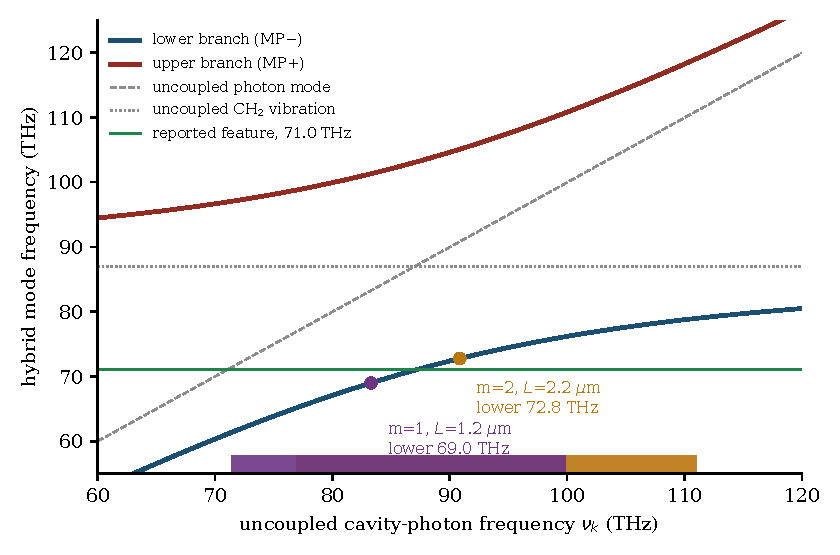
\includegraphics[width=0.82\textwidth]{fig_branches.pdf}
\caption{Hybrid-mode branches from Eq.~\eqref{eq:branches} with $t=16.04\thz$ and $\nu_{\mathrm{vib}}=87\thz$, against the uncoupled cavity-photon frequency. The two marked points are the preprint's two length classes evaluated at its stated $n=1.5$, with the one-standard-deviation range of length shown as a bar on the horizontal axis. \stD{} Under the stated inputs the lower branch is predicted at $72.8$ and $69.0\thz$ for the two classes and spreads over roughly $14\thz$ within each, against a reported common position of $71.0\thz$.}
\label{fig:branches}
\end{figure}

\stD{} Either the model is evaluated at its stated geometry, in which case it predicts tissue-dependent branch positions and a broad ensemble distribution that are not observed, or resonance is imposed at every mitochondrion regardless of its length, in which case the length-matching argument carries no explanatory weight and a separate mechanism is needed to hold the photon mode at 87\,THz. The refractive index is itself uncertain (the preprint uses a value cited from measurements on myelinated axons), and a different index shifts both predictions, but it cannot remove the distinction between the two length classes unless the index also differs between tissues in exactly the compensating way.

The existence of the confined mode is a further, separate, assumption. \stD{} For an interface between lipid of index 1.5 and an aqueous matrix of index in the range 1.36 to 1.40, the Fresnel reflectance is $R\approx1.2\times10^{-3}$ to $2.4\times10^{-3}$, and the Fabry--Perot finesse $\pi\sqrt R/(1-R)$ is about 0.11 to 0.15 (standard Fabry--Perot theory \cite{bornwolf}). These index values are assumptions of the present analysis, and mid-infrared water absorption is strong and would lower the quality further. A finesse well below unity means that a photon does not complete a round trip coherently, which is the opposite of cavity confinement. In addition, the reported diameters of $0.3$ to $1.6\,\mu\mathrm{m}$ are smaller than the in-medium wavelength of $2.3\,\mu\mathrm{m}$, so the field of a weakly guiding rod is not a plane wave along its axis, and a waveguide mode analysis would be needed. These points do not show that confinement is impossible. They show that the preprint offers no calculation or measurement of mode structure, lifetime, or quality factor, and that the elementary estimate points against it.

A last issue concerns emission. \stR{} The model text says that an excited CH$_2$ bond will emit an 87\,THz photon on relaxing (p.~8, preceded by ``in principle''). \stD{} For a transition dipole of $0.03$ to $0.1$\,D the spontaneous emission rate at 87\,THz, $A=16\pi^3\nu^3\mu^2/(3\varepsilon_0hc^3)$, is about 7 to $77\,\mathrm{s^{-1}}$, a radiative lifetime of 13 to 145\,ms, whereas vibrational relaxation of C--H stretching in condensed phase proceeds on timescales of order a picosecond. The radiative branching ratio is then of order $10^{-11}$ to $10^{-10}$ per excitation. Collective effects and cavity enhancement could raise this, but enhancement requires the quality factor that is not demonstrated. The picture in which vibrations repeatedly exchange real photons across the cavity therefore needs a quantitative account of the photon source.

\section{The Observed Response}
\label{sec:atp}

\subsection{What was measured}

\stR{} ATP was measured per cell in lysates of 3D cell clusters by a luciferase assay after 10 minutes of illumination. Control wells were untreated wells paired within a column, and statistics were by paired $t$-test with $n=8$ pairs. Reported changes are $+10.3\%$ ($p<0.001$) at 71.0\,THz, $+10.1\%$ ($p<0.01$) at 87.0\,THz, and no significant change ($p>0.05$) at 53.7\,THz at the same stated power density (pp.~11--12, Fig.~5). The design has virtues that should be acknowledged: pairing within a plate column controls for growth conditions, normalization is to cell number, and the 53.7\,THz arm is a genuine control for incident power that gives some protection against a purely nonspecific optical effect. It is also a single endpoint at a single time.

\subsection{Abundance is not synthesis flux}

\stD{} The measured quantity is accumulated ATP concentration $A$ at the time of lysis, which obeys $\dot A=J_{\mathrm{prod}}-J_{\mathrm{cons}}$ with possible redistribution among compartments. A positive change $\Delta A$ equals $\int(\Delta J_{\mathrm{prod}}-\Delta J_{\mathrm{cons}})\,dt$ and does not identify the sign of either term. A reduction in consumption alone, as from a transient decrease in ATP-demanding activity, gives $\Delta A>0$ with no change in synthesis, and a shift between oxidative phosphorylation and glycolysis can change production without changing the mitochondrial contribution. A minimal model shows the non-identifiability directly: for $\dot A=J_0-kA$, an increase of the steady state $A^*=J_0/k$ by ten percent is produced equally by a 10\% rise in $J_0$ or a 9\% fall in $k$. \stR{} The preprint repeatedly calls the result increased ATP production (pp.~11--12). The assay does not support that wording, only an increase in measured ATP.

\stP{} To identify production, the following would be informative: oxygen consumption and extracellular acidification during and after illumination, the ATP/ADP ratio, mitochondrial membrane potential, responses to inhibitors of the respiratory chain and ATP synthase, and time-resolved ATP read out by genetically encoded fluorescent sensors so that the kinetics of onset and decay are available. A regulated effect has a characteristic time course, and an endpoint measurement cannot distinguish it from a transient artefact.

\subsection{Dose and heat}

\stR{} The power is 10\,$\mu$W at the fibre tip over a spot of about 1\,mm, which the main text states as $10\,\mu\mathrm{W\,mm^{-2}}$. \stD{} A 1\,mm circular spot has an area of $0.79\,\mathrm{mm}^2$, giving about $13\,\mu\mathrm{W\,mm^{-2}}$, so the two statements are consistent at the stated precision. The energy delivered in 10 minutes is 6\,mJ. If all of it were absorbed in the roughly $8\,\mu\mathrm{L}$ of cluster and medium (3\,$\mu$L plus 5\,$\mu$L) with no loss, using $4.18\,\mathrm{J\,g^{-1}K^{-1}}$ for water, the mean temperature rise would be at most $0.18\,\mathrm{K}$. Assuming a temperature coefficient $Q_{10}=2$ for the relevant metabolic rate, this corresponds to a rate change of about 1.3\%, and reaching 10\% would require a uniform rise near 1.4\,K. This estimate cuts against the strongest form of a bulk-heating explanation, and it is recorded as such.

\stD{} It does not close the question, for three reasons. Absorption at these wavelengths is strong in water and lipid and differs by large factors between 3.45, 4.22, and 5.58\,$\mu$m, so the energy is deposited in a thin layer near the illuminated surface of the cluster, where local heating can greatly exceed the bulk mean. The preprint reports no temperature measurement and no measurement of absorbed power. And the beam passes through an incubator atmosphere of 5\% CO$_2$ (Supplementary Fig.~11), whose gas-phase absorption lies in the neighbourhood of 4.2\,$\mu$m ($2370\cmi$ for the 71\,THz line), so that delivered power at the sample may differ among the three wavelengths even though the fibre-tip power is nominally equal. Equal incident power at different wavelengths is therefore not equal absorbed dose. \stP{} The comparison needs absorbed power per unit volume, direct temperature measurements at the cluster surface (for example by thermocouple or temperature-sensitive fluorescent probes), and a heat-matched control, such as a wavelength outside the CH$_2$ band chosen to deposit the same absorbed power.

\subsection{Two frequencies, one effect, and three points}

\stR{} The 71\,THz result is attributed to resonance with the proposed mito-polariton and the 87\,THz result to resonant absorption of the CH$_2$ bond itself (p.~11--12). \stD{} The magnitudes are indistinguishable at 10.3\% and 10.1\%, so two different causal accounts are offered for one observed effect, and nothing in the experiment separates them. A resonant mechanism makes a richer prediction than three frequencies can test. If the response is controlled by a mode with width $\Gamma$ centred at $\nu^*$, then the response as a function of frequency should have a shape $A(\nu)-A_0\propto\mathcal L(\nu;\nu^*,\Gamma)$ whose position, width, and symmetry are linked to the spectral feature. Three points, one of which is a null in a spectral region with different absorption, constrain neither $\nu^*$ nor $\Gamma$. The finding that $53.7\thz$ gave no effect shows that not every mid-infrared frequency acts, and the finding that two frequencies acted shows that at least two do, but this is far from a response function.

\subsection{Efficiency, quantum, and information language}

\stR{} The introduction states that mitochondrial energy transduction efficiency ``can reach $\sim$90\%, already beyond the conventional framework of thermodynamics'', citing references 23 and 24 (p.~3). \stD{} By their titles, those works address the thermodynamic efficiency of ATP synthase and the thermodynamic efficiency, reversibility, and degree of coupling of the respiratory chain \cite{matta2015,wikstrom2020}. High efficiency in a biochemical energy converter is a statement about how much of the available free energy is conserved. It is established by an energy budget that is consistent with thermodynamics, and it does not place the converter outside thermodynamics. Three meanings of ``quantum'' are being used together: the quantization of molecular energy levels, which is ordinary molecular physics and uncontroversial; a coherent collective excitation, which is a specific physical hypothesis; and a functional quantum advantage, which is a comparative claim requiring evidence that the mechanism outperforms relevant classical alternatives. Evidence for the second does not supply the third. Further, an efficiency is a ratio of conserved output to input free energy, so a 10\% change in ATP abundance supplies the numerator of nothing: neither the input flux nor the output flux was measured, and no efficiency can be computed.

\stR{} The abstract and conclusion raise as a possibility that the state could act as a channel for energy metabolism and ``information transmission in life'' (pp.~2, 12). The preprint presents this as a direction for further exploration and contains no measurement bearing on it. A communication channel requires an identifiable source, a distinguishable signal, a receiver, and demonstration that variation in the transmitted variable changes the receiver's state in a reproducible and informative way. Formally, a channel from $s$ to $y$ requires $I(s;y)>0$ under variation of $s$ imposed by the system itself, but this is necessary and not sufficient, since statistical dependence also arises from a common cause. Establishing a channel needs causal dependence under intervention, a distinction developed in Section~\ref{sec:endo}.

\section{Perturbability, Selectivity, and Control}
\label{sec:control}

\subsection{Setting}

Suppose that the proposed mode exists and that stimulating it changes ATP abundance. The mechanism then has a set of tunable parameters $\theta=(\nu,I,\tau,L,n,\rho,\eta,T,\dots)$ for frequency, intensity, duration, organelle geometry, refractive index, oscillator density, dipole orientation, and temperature, and the biological response is some function $\Delta A=F(\theta,x_0)$ of those parameters and the initial physiological state $x_0$. ATP is one coordinate of a larger state vector,
\begin{equation}
x=\bigl([\mathrm{ATP}],[\mathrm{ADP}],\Delta\Psi_m,\mathrm{ROS},\mathrm{pH},[\mathrm{Ca}^{2+}],\mathrm{OCR},\dots\bigr)^{\!\top},
\end{equation}
and a general physical coupling that perturbs the mitochondrial system has no reason to perturb only one coordinate. A theory that explains an ATP increase by a general coupling is thereby committed to a statement about the other coordinates, including consequences that may be unwelcome to the functional interpretation, and it should not be allowed to count a change in ATP as evidence for a beneficial energy channel while treating changes elsewhere as irrelevant. The same commitment extends to the explanatory burden: if the model allows a broad family of tunable interventions, it must account for the whole response surface that its assumptions imply, not only the point selected for publication.

\subsection{Definitions}

Let each coordinate of $x$ be scaled by its physiological range, so that statements about relative size do not depend on units. Let $\Phi_\tau(x_0,\theta)$ be the state after exposure $\theta$ for duration $\tau$, with $\theta_0$ the unexposed condition, and write $\Delta x=\Phi_\tau(x_0,\theta)-\Phi_\tau(x_0,\theta_0)$ with $\Delta y=c^\top\Delta x$ the change in the measured coordinate.

\begin{definition}[Responsive]
The stimulus is \emph{responsive} for $y$ at $x_0$ if $\Delta y\ne0$ for some $\theta$.
\end{definition}

\begin{definition}[Selective]
The stimulus is \emph{selective with ratio $s$} for $y$ on a set $X_0$ of initial states and a set $\Theta_0$ of parameters if $|\Delta y|\ge s\,\|\Delta x_{\perp y}\|$ for all $x_0\in X_0$, $\theta\in\Theta_0$, where $\Delta x_{\perp y}$ is the vector of changes in all other coordinates.
\end{definition}

\begin{definition}[Independently controllable]
In the local linear model $\dot x=Ax+B\,u$, the coordinate $y$ is \emph{independently controllable} if the vector $e_y$ (the unit direction that changes $y$ alone) lies in the range of the controllability matrix
\begin{equation}
\mathcal C=\bigl[\,B,\;AB,\;A^2B,\;\dots,\;A^{n-1}B\,\bigr].
\end{equation}
\end{definition}

The three definitions are ordered by strength. Responsiveness concerns one coordinate in one condition. Selectivity adds the behaviour of all the other coordinates over specified ranges of state and parameter. Independent controllability concerns whether $y$ can be moved while the rest are held fixed, which requires sufficient rank of $\mathcal C$ and not merely a nonzero entry in $c^\top B$.

\subsection{What a single response licenses}

\begin{proposition}[A single response does not establish selectivity, controllability, or state independence]
\label{prop:single}
Let one exposure $(\theta_1,x_0)$ yield $\Delta y>0$. This observation is consistent with models in which (a) the stimulus is selective with ratio $s$ arbitrarily close to zero, (b) $y$ is not independently controllable, and (c) $\Delta y$ has the opposite sign at other initial states.
\end{proposition}

\begin{proof}
(a,b) Take $n=2$, $x=(y,z)^\top$, $A=-\lambda I$ with $\lambda>0$, and $B=(\epsilon,1)^\top$ with $\epsilon>0$ small. The response to a constant input $u$ for time $\tau$ is $\Delta x=\lambda^{-1}(1-e^{-\lambda\tau})\,u\,B$, so $\Delta y>0$ while $\|\Delta x_{\perp y}\|=|\Delta z|=\epsilon^{-1}\Delta y$, and the selectivity ratio is $\epsilon$. Moreover $\mathcal C=[B,\,-\lambda B]$ has rank one, with range spanned by $B$, which does not contain $e_y=(1,0)^\top$. (c) Take $\dot y=-\lambda(y-y^\dagger)+u\,(y-y^*)$ with $u>0$ and $y^*\ne y^\dagger$. The effect of $u$ on the rate of change of $y$ has the sign of $y-y^*$, so initial states on opposite sides of $y^*$ yield responses of opposite sign. Each model agrees with a single observation of $\Delta y>0$ at one chosen $x_0$.
\end{proof}

The proposition is not a claim that the ATP response in the preprint is non-selective or non-controllable. It is the statement that the observation does not decide the matter, so that selectivity has to be measured. It also allows the correct reading of the set-point objection: the existence of a tunable coupling does not imply arbitrary controllability, and the distinction between perturbability and controllability is the distinction between $\Delta y\ne0$ and the rank condition above. Framed that way, the demand on the authors is not that arbitrary control must follow from their model, but that a selectivity and controllability account must accompany a claim of control.

\begin{criterion}[Measurements that would support selective control]
\label{crit:support}
This is a methodological identification criterion, not a theorem: it does not follow from the definitions alone, and is proposed as the minimal evidential standard for the claim. A claim that illumination at frequency $\nu_0$ is a selective control channel for ATP, with ratio $s$ on $(\Theta_0,X_0)$, is supported only by data of four kinds: (E1) the response measured as a function of the parameters over $\Theta_0$, with shape linked to independently measured spectral parameters; (E2) simultaneous measurement of the other coordinates, from which the ratio in Definition~2 can be estimated; (E3) repetition across initial states in $X_0$ chosen to vary the relevant physiological variables; (E4) removal or alteration of the proposed structural basis, giving a change in the response that follows a prediction made in advance.
\end{criterion}

\stD{} The preprint supplies none of E1 to E3 for ATP, and for E4 it supplies a contrast in the spectral feature (Section~\ref{sec:obs}) and none in the response. This is an assessment of coverage and not a verdict on the underlying effect. \stR{} The preprint's own conclusion that the state ``provides an efficient channel to modulate ATP production'' (pp.~1, 11--12) is a statement of the fourth level, and the evidence offered belongs to the third.

\subsection{Exogenous capability and endogenous utilization}
\label{sec:endo}

The distinction between a response to an applied intervention and utilization of that intervention pathway by the system itself is separate from the question of selectivity and is a more general one.

\begin{proposition}[Exogenous response does not establish endogenous utilization]
\label{prop:endo}
Let $R:S\to Y$ be the map from a signal $s$ (here the in-band optical field) to a response $y$. An exogenous experiment applying $s_{\mathrm{exo}}$ and observing $\Delta y\ne0$ establishes only that $R$ is non-constant on a set containing $s_{\mathrm{exo}}$. Endogenous utilization of the same pathway additionally requires (U1) an endogenous field $s_{\mathrm{en}}$ present in the tissue within the region where $R$ is non-constant, at an amplitude distinguishable from the ambient background in that band; (U2) observational covariation of $y$ with natural variation of $s_{\mathrm{en}}$, formally $I(s_{\mathrm{en}};y)>0$ over physiological conditions, which is necessary but not sufficient because a common cause can generate dependence without any effect of $s_{\mathrm{en}}$ on $y$; and (U3) causal dependence, meaning an alteration of $y$ in the predicted direction when the source of $s_{\mathrm{en}}$ is intervened on, with relevant confounders controlled. None of U1 to U3 follows from the exogenous response.
\end{proposition}

\begin{proof}
Let $S=\{s_{\mathrm{en}},s_{\mathrm{exo}}\}$ with $R(s_{\mathrm{exo}})\ne R(s_0)$ and $R(s_{\mathrm{en}})=R(s_0)$, where $s_0$ is the unexposed value; the exogenous experiment shows a response while the endogenous field has no effect. The ionizing-radiation analogue is familiar: cells respond to ionizing radiation through damage-sensing pathways, and no one infers that those pathways exist to be regulated by ionizing radiation. For (U2), if $s_{\mathrm{en}}$ is constant over physiological conditions then $I(s_{\mathrm{en}};y)=0$ whatever the form of $R$; and if $s_{\mathrm{en}}$ and $y$ are both driven by a third variable $w$ (for example metabolic state) with $R$ constant at $s_{\mathrm{en}}$, then $I(s_{\mathrm{en}};y)>0$ with no utilization, so U2 cannot replace U3.
\end{proof}

This is the proposition for which the preprint is a near-ideal case, and it generalizes the distinction between an enabling condition and a demonstrated function of the companion essay: a response to an experimentally supplied intervention does not show that the system ordinarily exploits that pathway. Some quantities bear on U1. \stD{} The thermal background in the 71\,THz band at 310\,K is low. The mean photon occupation per mode is $\bar n=1/(e^{h\nu/k_BT}-1)=1.7\times10^{-5}$, because $h\nu/k_BT=11.0$ ($k_BT/h=6.5\thz$). Treating tissue as a blackbody, the in-band intensity in a $1\thz$ window emitted into a hemisphere is about $0.28\,\mu\mathrm{W\,mm^{-2}}$, so the stimulus of about $10$ to $13\,\mu\mathrm{W\,mm^{-2}}$ in a spectrally narrow line is some 35 to 45 times the thermal background even when the latter is integrated over a full terahertz. The low thermal occupation is the strongest physical reason that infrared-frequency signalling is not absurd on noise grounds, since a signal at 71\,THz is not drowned by thermal photons the way one at radio frequencies would be. It is not a demonstration of utilization. U1 also needs a source, and Section~\ref{sec:model} gives the radiative branching ratio that a CH$_2$ source would have without demonstrated enhancement. U2 and U3 need measurements that the preprint does not attempt.

\section{The Portability of Quantum Formalism and the Limits of Mechanistic Inference}
\label{sec:portability}

\subsection{Three things that are easily run together}

A mathematical formalism developed for one class of systems can be carried to another. Quantum mechanics is unusually portable in this respect, because its core structure (a state space, a Hamiltonian, eigenvalues, and superposition) applies to any system with two or more distinguishable alternatives and a coupling between them. This makes it important to separate three statements that are often fused. The first is that a system \emph{is} quantum, in the sense that its relevant dynamics are quantum-coherent. The second is that a quantum-like \emph{representation} reproduces the system's observed behaviour. The third is that evidence has been obtained that a specific mechanism operates through quantum coherence. The first and third are claims about the world, and the second is a claim about a model. The preprint's title makes the first claim and the evidence supports, at most, the second.

A useful contrast is supplied by a set of papers that apply two-level and tunnelling formalisms to the perception of ambiguous figures such as the Necker cube. In the sense used here they are a comparison class and not evidence about mitochondria: each of them is, on its face, a case in which quantum mathematics describes a system whose behaviour admits several interpretations, and they differ from one another and from the preprint in how much ontological weight they place on the mathematics. \stR{} Only summaries or abstracts of these three papers were examined, and statements about them below are at that level.

\subsection{Three cases}

\stR{} Maksymov (2023, arXiv:2312.03447) builds a neural network model of Necker-cube perception in which the connection weights are set from random numbers produced by a quantum source, and reports that the perceived state behaves like a qubit-like superposition of the two readings \cite{maksymov2023}. \stD{} Three separate questions are present: the physical origin of the random numbers, the mathematical representation of the output, and the physical mechanism of perception. Using randomness from a quantum device establishes the first of these and says nothing about the third, since the network's dynamics would be unchanged by drawing the weights from a classical pseudorandom generator with the same statistics. The representation of the output as a superposition is a statement about the representation.

\stR{} Benedek and Caglioti model the perception of the Necker cube as a two-level system modelled on the ammonia molecule's tunnelling doublet, with each orientation of the cube corresponding to a basis state, a coupling between them, and a symmetric and an antisymmetric combination split by an energy gap. They relate the perceptual oscillation frequency to the splitting through an effective neurophysiological action constant, which they estimate at about $2\,\mathrm{mJ\,s}$, and they describe the model as quantum-like and acknowledge that their energy estimates rest on macroscopic arguments that cannot shed light on synaptic-level mechanisms \cite{benedek2019}. \stD{} The two-by-two Hamiltonian is
\begin{equation}
H=\begin{pmatrix}E_0&E_r\\E_r&E_0\end{pmatrix},\qquad E_\pm=E_0\pm E_r,
\label{eq:necker}
\end{equation}
which has the same algebraic form as Eq.~\eqref{eq:branches} at resonance. The ratio of the quoted action constant to $\hbar$ is $2\times10^{-3}/1.05\times10^{-34}\approx2\times10^{31}$. A constant larger than Planck's by thirty-one orders of magnitude marks the formalism as an effective, phenomenological description whose parameters have no microscopic quantum interpretation, and the authors' own wording is consistent with that reading. The model nonetheless reproduces a perceptual oscillation, which is the point: representational adequacy is achieved by a formalism whose constants are not microscopic quantum constants.

\stR{} Maksymov and Pogrebna (2023) describe a harmonic-oscillator model, an electron in a potential well, applied to bistable perception, in which tunnelling through a barrier is compared with the eye blink, known to be associated with perceptual reversals, and the eye blink is offered as a viable physiological connection between the physics and the perception \cite{maksymov2023b}. \stD{} The structure is that of the previous case with a physiological candidate attached. The model's capacity to reproduce switching is a statement about representation, and the physiological link, on the account given by its authors, is an analogy offered for consideration, not a demonstrated mechanism. The full text was not available to the present analysis, so the extent to which the authors qualify this link is not assessed.

\subsection{A common structure and what it licenses}

All of these, together with the mitochondrial model, are instances of a general two-state operator
\begin{equation}
H(\theta)=\begin{pmatrix}E_1(\theta)&g(\theta)\\ g^*(\theta)&E_2(\theta)\end{pmatrix},\qquad
E_\pm=\frac{E_1+E_2}{2}\pm\sqrt{\frac{(E_1-E_2)^2}{4}+|g|^2}.
\label{eq:general}
\end{equation}
The resemblance is mathematically meaningful and carries no information about shared physical mechanism. A coupled pair of classical pendula, an LC circuit pair, the ammonia doublet, a double-well tunnelling system, a bistable perceptual state, and a light--matter hybrid all have Hamiltonians or normal-mode matrices of this form, and any observable defined through the spectrum alone takes the same values in all of them.

\begin{definition}[Representational adequacy and mechanistic identification]
A model $\mathcal M$ with parameters $\theta$ has \emph{representational adequacy} for data $D$ if some $\hat\theta$ reproduces $D$ within the tolerance of interest. It achieves \emph{mechanistic identification} if, in addition, (I1) the parameters are independently measured or constrained, (I2) each mathematical quantity corresponds to a physical quantity with matching units and a measurable meaning, and (I3) the model makes predictions that competing models cannot reproduce, which are tested.
\end{definition}

\begin{proposition}[Formal equivalence does not imply mechanistic equivalence]
\label{prop:portable}
Let $\mathcal M_1$ and $\mathcal M_2$ be models of different physical systems with Hamiltonians $H_1$ and $H_2$ that are unitarily equivalent. Then every observable that is a function of the spectrum alone has the same value in both, and data consisting only of such observables cannot discriminate the models.
\end{proposition}

\begin{proof}
If $H_2=UH_1U^\dagger$, the spectra coincide, and a function of the spectrum takes the same value for both. The models are defined on carriers with different physical interpretations (one possibility is a polariton, another a pair of coupled pendula), and nothing in the spectrum refers to the carrier.
\end{proof}

The proposition shows why the adequacy of a two-state model for a switching frequency, an energy splitting, or a response trajectory is weak evidence of mechanism. With sufficiently flexible choices of $E_1(\theta)$, $E_2(\theta)$, and $g(\theta)$ the form of Eq.~\eqref{eq:general} accommodates a wide range of splittings and switching rates. The scientific question is whether the parameters are independently constrained and whether the model predicts something its competitors do not, which is exactly the standard that Section~\ref{sec:model} applies to the mitochondrial coupling and that the Necker-cube models, in their own terms, do not claim to meet.

\subsection{Discriminating observables, and the standard applied back}

\stP{} For bistable perception, quantum-like models must be separated from classical stochastic and adaptation-based accounts, in which mutual inhibition between neural populations, slow adaptation, and noise produce alternation. Observables that discriminate include the dependence of dominance-duration statistics on stimulus strength and bias, sequential dependence between successive durations, and temporal inequalities of the Leggett--Garg type, which a coherent two-level system can violate under non-invasive measurement while a classical stochastic system cannot \cite{leggett1985}. The last has a known loophole, since the measurement of a percept may be invasive, so a failure to violate it is informative and a violation would need the invasiveness assumption addressed. None of this is supplied by the adequacy of a Hamiltonian fit.

\stD{} The same standard applies to the polariton, and it exposes a point that the title obscures. In linear response, the eigenvalue problem of Eq.~\eqref{eq:branches} is also the normal-mode problem of two coupled classical oscillators, and the classical Lorentz-medium treatment reproduces the same two branches and the same square-root dependence of the splitting on oscillator density. A measured avoided crossing, even one with all the properties demanded in Section~\ref{sec:model}, would therefore establish a hybrid normal mode, a result that is physically interesting and fully classical in its linear-response content. The qualifier ``quantum'' adds content only through observables that a classical description does not reproduce, for example photon statistics, nonlinear or time-resolved dynamics that depend on the quantized excitation number, or entanglement between the constituents. The preprint reports no such observable. This does not make the polariton hypothesis wrong or uninteresting. It means that the decisive discriminating tests for the word ``quantum'' are separate from the tests for the existence of the hybrid mode, and that Level~2 of Table~\ref{tab:levels} can be established without the quantum claim following.

Taken together, the comparison class supports the general proposition without implying that the mitochondrial mechanism is false. The proposed polariton is a physically specific hypothesis, with a named oscillator, a named cavity, and a quantitative prediction, and in that respect it makes a stronger and more testable claim than the effective two-level descriptions of perceptual switching. The mathematics does not, in either case, supply the authority that would justify the ontological conclusion. What supplies it is independent measurement of parameters, units that correspond to measurable quantities, and discriminating predictions that are tested and survive.

\section{Counterfactual Experiments}
\label{sec:cf}

\subsection{Accommodation and prediction}

A model accommodates an observation when its parameters are set after the observation so as to reproduce it. It predicts when its parameters are fixed by independent inputs and it then commits to the outcome of an experiment not yet performed. The distinction can be put in terms of residual degrees of freedom. \stD{} The preprint reports one spectral feature and one fitted-looking parameter $t$ (Section~\ref{sec:model}), which leaves no residual degrees of freedom: the model reproduces the feature because $t$ was chosen to do so, or because it was calculated from inputs that are not independently shown. This is not a charge of bad faith. It is the position of any model at the stage in which a first observation has suggested it, and it is the position from which a model has to move before it counts as explanatory.

The relevant constructive question is which experiments the model itself implies. The structure of Eq.~\eqref{eq:branches} supplies two kinds. If the structure is altered, the coupling changes by a predictable amount, so the branches should move together. If the chemical identity of the oscillator is altered, the bare frequency $\nu_0$ itself should move by a known ratio.

\subsection{Experiment A: structurally induced shift of the resonance}

\stD{} At resonance with fixed orientation factor and transition dipole, $t\propto\eta\sqrt\rho$, so that for a relative change of oscillator density $\kappa=\rho/\rho_0$ the branches are
\begin{equation}
\nu_\pm(\kappa)=\nu_0\pm t_0\sqrt\kappa,\qquad \nu_++\nu_-=2\nu_0\ \text{independent of }\kappa.
\label{eq:midpoint}
\end{equation}
The sum rule in Eq.~\eqref{eq:midpoint} does not depend on the absolute calibration of $t_0$ and can be tested without knowing it. The lower branch moves from $71$ to $74\thz$ if $t$ falls from $16.04$ to $13\thz$, which requires $\kappa=(13/16.04)^2=0.657$, a reduction of oscillator density of 34\%. The upper branch would then be at $100.0\thz$. Figure~\ref{fig:shift} gives the branch positions as a function of $\kappa$.

\begin{figure}[ht]
\centering
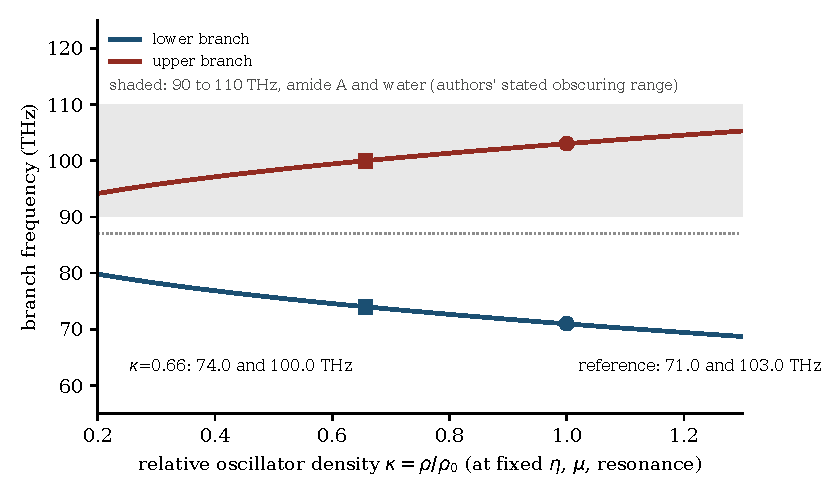
\includegraphics[width=0.82\textwidth]{fig_shift.pdf}
\caption{\stD{} Branch positions from Eq.~\eqref{eq:midpoint} as a function of relative oscillator density, at fixed resonance, orientation factor, and dipole. The marked square points correspond to $\kappa=0.657$, for which the lower branch is at $74.0\thz$ and the upper at $100.0\thz$. The shaded band is the range the authors give for obscuration by amide A and water.}
\label{fig:shift}
\end{figure}

\stP{} The experiment is to alter cristae organization or lipid composition under conditions that retain enough mitochondrial function for comparison, for example by genetic or pharmacological perturbation of cristae-shaping proteins or by controlled changes of acyl-chain composition, and to measure the structural variable independently (cristae spacing by electron or super-resolution microscopy, lipid composition by lipidomics, mitochondrial length by the same confocal method used in the preprint). The prediction is then computed from the full expression of Eq.~\eqref{eq:branches} with the measured $L$ and $n$, so that changes in detuning are included, and it is recorded before the spectra are acquired. The test has two parts, because two claims are being tested: the first is that the spectral feature shifts as predicted, and the second is that the maximum of the ATP response follows it. If the lower spectral branch moves from $71$ to $74\thz$, the decisive question is whether the maximum of $A(\nu)$ moves to the same place. Table~\ref{tab:outcomes} lists the four combinations.

\begin{table}[ht]
\centering
\small
\begin{tabularx}{\textwidth}{@{}p{3.1cm}p{3.1cm}X@{}}
\toprule
Spectral feature & ATP response maximum & Interpretation \\
\midrule
Shifts as predicted before measurement & Follows the shifted position & The polariton interpretation is considerably strengthened, in particular if the shift also agrees with independently measured structural parameters and the midpoint rule of Eq.~\eqref{eq:midpoint} holds. \\
Shifts as predicted & Stays at 71\,THz & The coupling between the spectral mode and the ATP response is weakened; the response may arise from a different pathway such as direct CH$_2$ absorption. \\
Shifts but not as predicted & Either & The spectral feature depends on structure but the quantitative model is wrong; the model should be revised, not defended. \\
Does not shift & Either & The structural dependence the model asserts is not present; the feature may have another origin. \\
\bottomrule
\end{tabularx}
\caption{\stP{} Outcomes of the structural-shift experiment and their interpretation. Each cell is defined in advance by the prediction computed from measured structural variables.}
\label{tab:outcomes}
\end{table}

\subsection{Experiment B: isotopic substitution of the oscillator}

A sharper test replaces the oscillator and not its density. \stD{} If lipid acyl chains are deuterated, the CH$_2$ stretch is replaced by a CD$_2$ stretch. The reduced-mass ratio for C--H and C--D is $(12\cdot2/14)/(12\cdot1/13)=1.857$, with square root $1.363$, so $\nu_{\mathrm{vib}}$ falls from $87$ to about $63.8\thz$. The prediction depends on what the cavity does. Isotopic substitution changes the oscillator and not the geometry, so, if the photon mode is set by the organelle length and the refractive index, which are unchanged to first order, the cavity stays at $\nu_c$ and the system becomes detuned, with $\delta=\nu_c-\nu_{\mathrm{vib}}\approx+23\thz$. The branches then follow the full expression
\begin{equation}
\nu_\pm=\frac{\nu_c+\nu_{\mathrm{vib}}}{2}\pm\sqrt{\left(\frac{\nu_c-\nu_{\mathrm{vib}}}{2}\right)^2+g^2},
\label{eq:detuned}
\end{equation}
with $g$ the coupling in the deuterated medium, which is unknown (the CD$_2$ dipole and oscillator strength are not given here), so illustrative values of $8$, $12$, and $16\thz$ are used. Table~\ref{tab:isotope} gives the results for the two cavity frequencies of interest.

\begin{table}[ht]
\centering
\small
\begin{tabular}{@{}ccccc@{}}
\toprule
 & \multicolumn{2}{c}{$\nu_c=87\thz$} & \multicolumn{2}{c}{$\nu_c=90.85\thz$} \\
\cmidrule(lr){2-3}\cmidrule(lr){4-5}
$g$ (THz) & lower & upper & lower & upper \\
\midrule
8 & 61.3 & 89.5 & 61.6 & 93.0 \\
12 & 58.7 & 92.1 & 59.3 & 95.4 \\
16 & 55.7 & 95.2 & 56.4 & 98.3 \\
\bottomrule
\end{tabular}
\caption{\stP{} Predicted branch positions (THz) after CD$_2$ substitution with the cavity held fixed at the pre-substitution frequency, from Eq.~\eqref{eq:detuned} with $\nu_{\mathrm{vib}}=63.84\thz$. The coupling $g$ is illustrative and unmeasured.}
\label{tab:isotope}
\end{table}

\stD{} Three features of this prediction are valuable. First, features derived from CO$_2$ (gas, dissolved, or otherwise) do not depend on the lipid isotopologue, so an artefact near 71\,THz should stay put while a polariton derived from CH$_2$ should leave: with the cavity fixed the lower branch moves to between about $56$ and $62\thz$ for $g=8$ to $16\thz$. Second, the model predicts a specific pattern, a lower branch that moves by roughly $9$ to $15\thz$ and an upper branch that moves much less, and a reported shift that departs from that pattern is informative. Third, the upper branch does not land in a spectrally unobscured window: it stays in the $89$ to $98\thz$ range, near the residual CH stretching bands of proteins and non-deuterated lipids and the edge of the amide A and water region, so the substitution does not by itself make the upper branch observable. The lower branch lies near the amide~I region, so subtraction against non-deuterated controls is needed. \stP{} An optional double-tuning variant retunes the cavity with the oscillator, by swelling the organelle so that $L$ increases by the factor $1.363$ (osmotic swelling of isolated mitochondria is an established manipulation, though its effect on the optical mode is untested); the resonance condition is then restored and branches fall at $\nu_{\mathrm{vib}}\pm g$. Practical difficulties include partial deuteration, which produces mixtures of isotopologues, and altered membrane properties, but these are difficulties of execution and do not alter the logic.

\subsection{Experiment C: the response function}

\stP{} A tunable source should be used to measure ATP as a function of frequency over a range that includes both branches and the bare vibration, with the response normalized to absorbed power measured in the sample, temperature recorded at the cluster surface, and flux-related observables recorded as in Section~\ref{sec:atp}. The prediction is a response whose position and width follow the independently measured spectral feature, $A(\nu)-A_0\propto\mathcal L(\nu;\nu^*,\Gamma)$ with $\nu^*=\nu_-$ and $\Gamma$ comparable to the measured linewidth. A flat or monotone response, or one whose maximum sits at the bare vibration, would indicate that the response is driven by direct absorption. The paired design of the original work is a good basis for this, and the 53.7\,THz point can be retained as one sample of the baseline.

Taken together, the three experiments convert a mechanism that is supported by one observation into one that makes testable commitments about a response surface. They also function as a diagnostic of what kind of theory is being offered: a theory that can name in advance where the feature and the response will go when a structural variable is changed is explanatory in a sense that a theory that can only point back to the first feature is not.

\section{Ledger and Relation to Companion Work}
\label{sec:ledger}

Table~\ref{tab:ledger} collects the claims examined, with their status, basis, and what would change that status. The point of a ledger of this kind is that each row names its own defeat condition, so that the argument remains open to correction by the data it asks for.

\begingroup
\small
\begin{longtable}{@{}p{0.5cm}p{4.6cm}p{0.8cm}p{3.3cm}p{3.4cm}@{}}
\toprule
ID & Statement & Tag & Basis & What would change the status \\
\midrule
\endfirsthead
\toprule
ID & Statement & Tag & Basis & What would change the status \\
\midrule
\endhead
C1 & A 71.0\,THz shoulder is present in ATR spectra of living preparations and absent in dried KBr-transmission spectra & \stR & Figs.~1--2, Methods p.~13 & Matched geometry, hydration, and atmosphere across preparations \\
C2 & The shoulder is not assignable to CO$_2$ or any known molecule & \stA & pp.~5, 23 & Purged ATR; $^{13}$CO$_2$ labelling; gas-phase reference at matched resolution \\
C3 & The two-mode Hamiltonian has branches $87\pm t$ & \stD & Eqs.~1--6; algebra verified & Not in question \\
C4 & $t\approx6.4\kjm$ follows from the structure & \stA & Eq.~4; $\mu$ unreported & Reported $\mu$ and $\rho$; band-strength calibration; density audit resolved \\
C5 & Stated density is inconsistent with stated bond spacing by about $8\times10^{3}$ & \stD & p.~8; polyethylene reference & Authors' clarification of the figure \\
C6 & Collective coupling implied by oscillator strength for CH$_2$ media is near 1--2\,THz under assumed absorption values & \stD & Table~\ref{tab:bound}; approximate inputs & Measured integrated absorbance of the authors' samples \\
C7 & The mitochondrion supports a confined 87\,THz photon mode & \stA & pp.~8, 10--11 & Mode and quality-factor measurement or calculation \\
C8 & Branch position is common across tissues at 71.0\,THz & \stR & Figs.~1--2 & Not in question as a report \\
C9 & The model at its stated inputs predicts 72.8 and 69.0\,THz for the two length classes and a roughly 14\,THz spread & \stD & Figs.~4 and \ref{fig:branches} & Evidence of compensating index or forced resonance \\
C10 & ATP per cell rises about 10\% at 71 and 87\,THz and not at 53.7\,THz & \stR & Fig.~5, $n=8$ pairs & Replication with kinetics and further controls \\
C11 & The increase reflects increased ATP production & \stA & pp.~11--12 & Flux, oxygen consumption, and ATP/ADP measurements \\
C12 & The effect is not thermal & \stA & Low stated power & Absorbed dose and surface temperature; heat-matched control \\
C13 & Bulk heating alone gives at most about 0.2\,K & \stD & 6\,mJ into about 8\,$\mu$L & Spatially resolved temperature data \\
C14 & The state is a selective channel for ATP modulation & \stA & pp.~1, 12 & E1 to E4 of Criterion~\ref{crit:support} \\
C15 & Cells use the mode endogenously for energy metabolism or information & \stA & Posed as open question & U1 to U3 of Proposition~\ref{prop:endo} \\
C16 & Efficiency near 90\% lies beyond thermodynamics & \stA & p.~3 & Energy-budget analysis showing a violation, which none of the cited works claims \\
C17 & A measured avoided crossing would establish a hybrid normal mode, which in linear response is also the classical coupled-oscillator result & \stD & Eq.~\eqref{eq:branches}; Section~\ref{sec:portability} & Observables that a classical description does not reproduce (photon statistics, quantized nonlinear dynamics) \\
C18 & Quantum-like two-state models of bistable perception show representational adequacy without mechanistic identification & \stD & Abstract-level summaries of three papers; Eq.~\eqref{eq:necker} & Independently constrained parameters and discriminating tests against adaptation and noise models \\
\bottomrule
\caption{Claims ledger with provenance tags.}
\label{tab:ledger}
\end{longtable}
\endgroup

Several lines of the analysis connect to other essays in the same programme, and it is useful to say how without repeating them. The enabling-condition versus demonstrated-function distinction of the companion essay is the backbone of Propositions~\ref{prop:single} and~\ref{prop:endo} and Criterion~\ref{crit:support}, extended here from the question of whether a function has been shown to the question of whether a controllable response licenses either control or utilization. The distinction between a formal model that reproduces an observation and one that corresponds to the physical system, treated in the work on verification without correspondence, appears in Section~\ref{sec:model}, where a coupled-mode Hamiltonian with correct algebra is separated from the physical assumptions that would make it apply. The cavity argument depends on average mitochondrial length, and resonance is sensitive to the individual geometry; the work on what averaging discards bears directly on that, and Section~\ref{sec:model} converts it into a quantitative prediction by replacing a mean length with a distribution. The question of where a domain of admissible explanations is closed is relevant to the preprint's treatment of the 71.0\,THz shoulder as unassignable, since the assignment is closed before alternatives such as atmospheric CO$_2$ and preparation differences have been excluded.

\section{Conclusion}

The spectral measurements in the preprint are worth replicating, the illumination result is worth investigating, and polariton physics is a legitimate framework for collective molecular excitations. The strongest claims are not established by what is reported. The shoulder is separated from a neighbouring gas-phase band by fitting, and the preparations that carry the contrast differ in several variables at once. The coupled-mode model has correct algebra, but its coupling strength is not fixed by independent inputs, its stated density is inconsistent with its stated bond spacing, an oscillator-strength consistency constraint, under assumed absorption values that need independent sourcing, places the implied coupling roughly an order of magnitude below the value needed, and at its own geometry it predicts tissue-dependent positions that are not reported. The ATP result is a measured change in abundance and not in production, and a single response of one variable to one stimulus establishes neither selectivity, independent controllability, nor endogenous use.

The general conclusion is the one stated in Propositions~\ref{prop:single} and~\ref{prop:endo} and Criterion~\ref{crit:support}: a demonstrated response to an intervention does not establish a functional control channel unless its selectivity, its operating limits, and its dependence on the initial state are independently characterized, and it does not establish endogenous utilization without evidence on source, covariation, and removal. If the model admits a broad family of tunable electromagnetic interventions, its explanatory burden increases, since it must account for the whole response surface that its assumptions imply. The comparison with quantum-like models of perceptual switching in Section~\ref{sec:portability} adds that the adequacy of a two-state Hamiltonian for a switching frequency or a splitting is weak evidence of mechanism, and that the word ``quantum'' needs observables that a classical coupled-oscillator description does not supply. The structural-shift and isotope experiments of Section~\ref{sec:cf} are constructive because they ask the proposed mechanism to say in advance where a feature and a response will go, and they would be informative whichever way they came out.

\begin{thebibliography}{99}
% Provenance: yang2026, matta2015, wikstrom2020 checked against the preprint; maksymov2023 against arXiv 2312.03447; hopfield1958, kockum2019, forndiaz2019, leggett1985, bornwolf matched to publication records in a check supplied by the author (not independently repeated here).
\bibitem{yang2026} Yang, Y., Gu, Z., and Song, B. A quantum state of mitochondria in the living cell. \emph{bioRxiv} (posted 15 September 2026), doi:10.64898/2026.09.10.750628. Preprint, not peer reviewed.
\bibitem{hopfield1958} Hopfield, J. J. Theory of the contribution of excitons to the complex dielectric constant of crystals. \emph{Phys. Rev.} \textbf{112}, 1555--1567 (1958).
\bibitem{kockum2019} Kockum, A. F., Miranowicz, A., De Liberato, S., Savasta, S., and Nori, F. Ultrastrong coupling between light and matter. \emph{Nat. Rev. Phys.} \textbf{1}, 19--40 (2019).
\bibitem{forndiaz2019} Forn-D\'iaz, P., Lamata, L., Rico, E., Kono, J., and Solano, E. Ultrastrong coupling regimes of light-matter interaction. \emph{Rev. Mod. Phys.} \textbf{91}, 025005 (2019).
\bibitem{maksymov2023} Maksymov, I. S. Quantum-inspired neural network model of optical illusions. arXiv:2312.03447 (submitted 6 December 2023).
\bibitem{benedek2019} Benedek, G. and Caglioti, G. Graphics and quantum mechanics: the Necker cube as a quantum-like two-level system. In L. Cocchiarella (ed.), \emph{Proceedings of the 18th International Conference on Geometry and Graphics}, Springer (2019), pp.~161--172 (also listed as \emph{Advances in Intelligent Systems and Computing} \textbf{809}).
\bibitem{maksymov2023b} Maksymov, I. S. and Pogrebna, G. Linking physics and psychology of bistable perception using an eye blink inspired quantum harmonic oscillator model. arXiv:2307.08758 (2023); the arXiv record may carry a later title. Not published in a journal as far as examined, and consulted through an indexed abstract only.
\bibitem{leggett1985} Leggett, A. J. and Garg, A. Quantum mechanics versus macroscopic realism: is the flux there when nobody looks? \emph{Phys. Rev. Lett.} \textbf{54}, 857--860 (1985).
\bibitem{bornwolf} Born, M. and Wolf, E. \emph{Principles of Optics}, 7th ed. Cambridge University Press (1999).
\bibitem{matta2015} Matta, C. F. and Massa, L. Energy equivalence of information in the mitochondrion and the thermodynamic efficiency of ATP synthase. \emph{Biochemistry} \textbf{54}, 5376--5378 (2015).
\bibitem{wikstrom2020} Wikstr\"om, M. and Springett, R. Thermodynamic efficiency, reversibility, and degree of coupling in energy conservation by the mitochondrial respiratory chain. \emph{Commun. Biol.} \textbf{3}, 451 (2020).
\end{thebibliography}

\appendix
\section{Computation Record}

The numerical results used in the text, with formulas and inputs, are collected for reproducibility. All are \stD{} items and depend on the listed inputs.

\begin{table}[ht]
\centering
\small
\begin{tabularx}{\textwidth}{@{}p{3.3cm}p{4.2cm}X@{}}
\toprule
Quantity & Formula & Inputs and result \\
\midrule
Unit conversions & $h=0.39903\kjm\thz^{-1}$; $1\thz=33.356\cmi$ & $6.4\kjm=16.04\thz$; $0.2\thz=6.67\cmi$; $71.0\thz=2368\cmi$ \\
Branches at resonance & $\nu_0\pm t/h$ & $87\pm16.04$ gives $70.96$ and $103.04\thz$; $t/\nu_0=0.184$ \\
Orientation factor & $\eta_{\mathrm{eff}}=1/\sqrt2$ for isotropic in-plane dipoles & $t=11.34\thz$; branches $75.66$ and $98.34\thz$ \\
Cavity photon frequency & $\nu_k=mc/2nL$, $n=1.5$ & $90.8\thz$ ($m=2$, 2.2\,$\mu$m); $83.3\thz$ ($m=1$, 1.2\,$\mu$m); spacings $45.4$, $83.3\thz$ \\
Lower branch vs detuning & Eq.~\eqref{eq:branches}, $t=16.04\thz$ & $72.8$ (2.2\,$\mu$m); $69.0$ (1.2\,$\mu$m); $65.1$ to $79.0$ for $L=2.6$ to $1.8\,\mu$m; $61.3$ to $76.2$ for $L=1.4$ to $1.0\,\mu$m \\
Density audit & $1/d^2$; $60/(0.65\,\mathrm{nm}^2)$; $\rho_{\mathrm{PE}}=0.95\,N_A/14.03$ & $10^{8}\,\mu\mathrm{m}^{-2}$; $9.2\times10^{7}\,\mu\mathrm{m}^{-2}$; bulk $1.8\times10^{9}\,\mu\mathrm{m}^{-3}$; polyethylene $4.1\times10^{10}\,\mu\mathrm{m}^{-3}$; ratio to preprint bulk $245$ \\
Collective coupling & $t=\mu\sqrt{h\nu\rho/2\varepsilon}$, $\varepsilon_r=2.25$ & Dipole needed for $6.4\kjm$: $0.027$\,D at $10^{31}\,\mathrm{m}^{-3}$; $1.97$\,D at $1.8\times10^{27}\,\mathrm{m}^{-3}$ \\
Oscillator-strength consistency constraint & $\varepsilon''_{\mathrm{pk}}=2n\alpha\lambda_0/4\pi=\nu_p^2/(\Gamma\nu_0)$; $t/h=\nu_p/2\sqrt{\varepsilon_\infty}$ & $n=1.45$, $\varepsilon_\infty=2.1$, $\Gamma=20\cmi$, $\nu_0=2900\cmi$ (unsourced, order of magnitude); $t=0.70$, $1.22$, $2.22\thz$ for $\alpha=10^3$, $3\times10^3$, $10^4\cmi$ \\
Finesse & $R=((n_1-n_2)/(n_1+n_2))^2$; $\mathcal F=\pi\sqrt R/(1-R)$ & $n_1=1.5$; $n_2=1.36$ to $1.40$; $R=1.2\times10^{-3}$ to $2.4\times10^{-3}$; $\mathcal F=0.11$ to $0.15$ \\
Radiative rate & $A=16\pi^3\nu^3\mu^2/(3\varepsilon_0hc^3)$ & $\nu=87\thz$; $\mu=0.03$, $0.05$, $0.10$\,D: $A=6.9$, $19$, $77\,\mathrm{s^{-1}}$ \\
Heating bound & $\Delta T=P\tau/(c_p m)$ & $P=10\,\mu$W, $\tau=600$\,s, $m=8$\,mg: $\Delta T=0.18$\,K; $Q_{10}=2$ rate change $1.3\%$ \\
Thermal occupation & $\bar n=(e^{h\nu/k_BT}-1)^{-1}$; $B_\nu=2h\nu^3\bar n/c^2$ & $T=310$\,K, $71\thz$: $h\nu/k_BT=10.99$; $\bar n=1.68\times10^{-5}$; $0.28\,\mu\mathrm{W\,mm^{-2}}$ in $1\thz$ (hemisphere, unit emissivity) \\
Structural-shift prediction & $\nu_\pm=\nu_0\pm t_0\sqrt\kappa$ & $\kappa=0.657$: $74.0$ and $100.0\thz$ \\
Isotopic shift & $\nu_{\mathrm{CD}}/\nu_{\mathrm{CH}}=\sqrt{\mu_{\mathrm{CH}}/\mu_{\mathrm{CD}}}$ & $1/1.363$; $\nu_{\mathrm{vib}}'=63.84\thz$; cavity fixed at $87$: for $g=8,12,16\thz$ lower $61.3,58.7,55.7$, upper $89.5,92.1,95.2\thz$ (Eq.~\ref{eq:detuned}) \\
\bottomrule
\end{tabularx}
\caption{Computation record.}
\end{table}

\end{document}
